%%% Exemplo de utilização da classe ITA
%%%
%%%   por        Fábio Fagundes Silveira   -  ffs [at] ita [dot] br
%%%              Benedito C. O. Maciel     -  bcmaciel [at] ita [dot] br
%%%              Giovani Volnei Meinertz   -  giovani [at] ita [dot] br
%%%    	         Hudson Alberto Bode       -  bode [at] ita [dot]br
%%%    	         P. I. Braga de Queiroz    -  pi [at] ita [dot] br
%%%    	         Jorge A. B. Gripp         -  gripp [at] ita [dot] br
%%%    	         Juliano Monte-Mor         -  jamontemor [at] yahoo [dot] com [dot] br
%%%    	         Tarcisio A. B. Gripp      -  tarcisio.gripp [at] gmail [dot] com
%%%
%%%   Versão para overleaf:
%%%   por           Alejandro A. Rios Cruz - aarc.88@gmail.com
%%%                 Saulo Gómez            - sagomezs@unal.edu.co
%%%  IMPORTANTE: O texto contido neste exemplo nao significa absolutamente nada.  :-)
%%%              O intuito aqui eh demonstrar os comandos criados na classe e suas
%%%              respectivas utilizacoes.
%%%
%%%  Tese.tex  2016-08-25
%%%  $HeadURL: http://www.apgita.org.br/apgita/teses-e-latex.php $
%%%
%%% ITALUS
%%% Instituto Tecnológico de Aeronáutica --- ITA, Sao Jose dos Campos, Brasil
%%%                   http://groups.yahoo.com/group/italus/
%%% Discussion list: italus {at} yahoogroups.com
%%%
%++++++++++++++++++++++++++++++++++++++++++++++++++++++++++++++++++++++++++++++
% Para alterar o TIPO DE DOCUMENTO, preencher a linha abaixo \documentclass[?]{?}
%   \documentclass[tg]{ita}			= Trabalho de Graduacao
%   \documentclass[tgfem]{ita}	= Para Engenheiras
%   								msc     		= Dissertacao de Mestrado
%   								mscfem   		= Para Mestras
%   								dsc      		= Tese de Doutorado
%   								dscfem   		= Para Doutoras
%   								quali    		= Exame de Qualificacao
%   								qualifem 		= Exame de Qualificacao para Doutoras
% Para 'Draft Version'/'Versao Preliminar' com data no rodape, adicionar 'dv':
%   \documentclass[dsc, dv]{ita}
% Para trabalhos em Inglês, adicionar 'eng':
%   \documentclass[dsc, eng]{ita}
%		\documentclass[dsc, eng, dv]{ita}
%++++++++++++++++++++++++++++++++++++++++++++++++++++++++++++++++++++++++++++++
\documentclass[tg]{ita}    % ITA.cls based on standard book.cls
% Quando alterar a classe, por exemplo de [msc] para [msc, eng]) rode mais uma vez o botão BUILD OUTPUT caso haja erro
\usepackage{ae}
\usepackage{graphicx}
\usepackage{epsfig}
\usepackage{amsmath}
\usepackage{amssymb}
\usepackage{subfig}
\usepackage{multirow}
\usepackage{float}
\usepackage{amsthm}
\usepackage{url}         % formats URL addresses properly
\usepackage{appendix}    % allows appendix section to be included
\usepackage{lscape}      % allows a page to be rendered in landscape mode
\usepackage{multicol}    % allows text in multi columns
\usepackage{cancel}      % needed to show canceled terms in equations
\usepackage{lettrine}
\usepackage{float}
\usepackage{placeins}
\usepackage[outputdir=latex.out]{minted}
\usepackage{prettyref}

\renewcommand\listingscaption{Código}

\newrefformat{anex}{Anexo~\ref{#1}}
\newrefformat{lst}{Código~\ref{#1}}

% Make ref autocomplete work.
\newcommand{\cref}[1]{\prettyref{#1}}

\usemintedstyle{friendly}

%HHHHHHHHHHHHHHHHHHHHHHHHHHHHHHHHHHHHHHHHHHHHHHHHHHHHHHHHHHHHHHHHHHHHHHHHHHHHHHHHHHHHHHHHHHHHHHHHHHHHHHHHHHHH
%\usepackage{subfigure}
%\usepackage{subfigmat}
%PACOTEFIGURAS_SE _ERRADO_ESXCLUIR_ACIMA
\usepackage{booktabs}
%PACOTETABELAS_SE _ERRADO_ESXCLUIR_ACIMA
%HHHHHHHHHHHHHHHHHHHHHHHHHHHHHHHHHHHHHHHHHHHHHHHHHHHHHHHHHHHHHHHHHHHHHHHHHHHHHHHHHHHHHHHHHHHHHHHHHHHHHHHHHHHH

%++++++++++++++++++++++++++++++++++++++++++++++++++++++++++++++++++++++++++++++
% Espaçamento padrão de todo o documento
%++++++++++++++++++++++++++++++++++++++++++++++++++++++++++++++++++++++++++++++
\onehalfspacing

%singlespacing Para um espaçamento simples
%onehalfspacing Para um espaçamento de 1,5
%doublespacing Para um espaçamento duplo

%++++++++++++++++++++++++++++++++++++++++++++++++++++++++++++++++++++++++++++++
% Identificacoes (se o trabalho for em inglês, insira os dados em inglês)
% Para entradas abreviadas de Professora (Profa.) em português escreva: Prof$^\textnormal{a}$.
%++++++++++++++++++++++++++++++++++++++++++++++++++++++++++++++++++++++++++++++
\course{Engenheria da Computação}

% Autor do trabalho: Nome Sobrenome
\authorgender{masc}
\author{Luis Cláudio Magalhães de}{Holanda}
\itaauthoraddress{Rua Engenheiro Prudente Merieles de Morais}{12.243-750}{São José dos Campos--SP}

% Titulo da Tese/Dissertação
\title{Aplicação de Model Driven Development para o aumento de eficiência de um time de desenvolvimento e do serviço Web construído}

% Orientador
\advisorgender{masc}
\advisor{Prof.~Dr.}{Fábio Carneiro Mokarzel}{ITA}

% Coorientador
\coadvisorgender{masc}
\coadvisor{Prof.~Dr.}{Inaldo Capistrano Costa}{ITA}

%Coordenador do curso no caso de TG
\bosscoursegender{masc}
\bosscourse{Prof.~Dr.}{Johnny Marques}

% Palavras-Chaves informadas pela Biblioteca -> utilizada na CIP
\kwcip{Cupim}
\kwcip{Dilema}
\kwcip{Construção}

% membros da banca examinadora

\examiner{Prof. Dr.}{Alan Turing}{Presidente}{ITA}
\examiner{Prof. Dr.}{Linus Torwald}{}{UXXX}
\examiner{Prof. Dr.}{Richard Stallman}{}{UYYY}
\examiner{Prof. Dr.}{Donald Duck}{}{DYSNEY}
\examiner{Prof. Dr.}{Mickey Mouse}{}{DISNEY}

% Data da defesa (mês em maiúsculo, se trabalho em inglês, e minúsculo se trabalho em português)
\date{5}{março}{2021}

% Número CDU - (somente para TG)
\cdu{XXX.XX}

% Glossario
\makeglossary
\frontmatter

\begin{document}
% Folha de Rosto e Capa para o caso do TG
\maketitle

% Dedicatoria: Nao esqueca essa secao  ... :-)
\begin{itadedication}
Aos amigos da Graduação e Pós-Graduação do ITA por motivarem tanto a criação deste template pelo Fábio Fagundes Silveira quanto por motivarem a mim e outras pessoas a atualizarem e aprimorarem este excelente trabalho.
\end{itadedication}

% Agradecimentos
\begin{itathanks}
Agradeço meus pais, que sempre me apoiaram no caminho que quis seguir, minha irmã
e aos meus amigos, por todo o apoio emocional e moral.

Agradeço também a todos os professores que, de uma forma ou de outra, contribuiram
para o meu desenvolvimento intelectual que me permitiu produzir esse trabalho.

Por fim, agradeço ao time da TerraMagna, que abriu espaço para o desenvolvimento desse
trabalho durante o meu expediente e forneceu insumos para que realizasse os experimentos
necessários.

\end{itathanks}

% Epígrafe
\thispagestyle{empty}
\ifhyperref\pdfbookmark[0]{\nameepigraphe}{epigrafe}\fi
\begin{flushright}
\begin{spacing}{1}
\mbox{}\vfill
{\sffamily\itshape
``Doing the same thing repeatedly, and expecting \\
different results is the definition of insanity''\\}
--- \textsc{Albert Einstein}

\end{spacing}
\end{flushright}

% Resumo
\begin{abstract}
\noindent
Sistemas Web apresentam um grau de complexidade bastante diversificado, variando desde
um sistema comercial de um mercado de bairro até o sistema completo de uma multi-nacional
em escala global. Para simplificar o desenvolvimento desses sistemas, diversas ferramentas
foram desenvolvidas.

Este trabalho apresenta um novo modelo de gerador de APIs, com o objetivo de solucionar
problemas que ferramentas atuais apresentam. Esses problemas são relacionados a baixa
integração com outras ferramentas de desenvolvimento, como Object-Relational Mappings
(ORMs) e validadores. Mostramos também que o uso de um gerador que integre eficientemente
com o restante do ecossistema pode resultar em grandes ganhos de eficiência para o time de
desenvolvimento, além de abrir portas para o uso de outras ferramentas que não seriam possíveis
sem ele. Uma motivação para esse trabalho é a busca do aumento de eficiência e automação dentro
do processo de desenvolvimento e a redução na incidência de defeitos em sistemas complexos.

\end{abstract}

% Abstract
\begin{englishabstract}
\noindent
This work presents a new model of API generator, intending to solve problems that
current solutions have. These problems are related to low integration with other
development tools such as ORMs and validators. We also show that the use of a
generator integrating effectively with the rest of the ecosystem can result in
significant efficiency gains for a development team and open doors for the use of
other tools that would not be possible without it. One motivation for this work
is to search for increased efficiency and automation within the development process
and reduce defects in complex systems.

\end{englishabstract}

% Lista de figuras
\listoffigures %opcional

% Lista de tabelas
\listoftables %opcional

% Lista de abreviaturas
\listofabbreviations
\begin{longtable}{ll}
  API & \textit{Application Programming Interface} \\
  IDL & \textit{Interface Definition Language} \\
  ORM & \textit{Object-Relational Mapping} \\
\end{longtable}

 %opcional

% Lista de simbolos
\listofsymbol
\begin{longtable}{ll}
\end{longtable}

 %opcional

% Sumario
\tableofcontents


\mainmatter
% Os capitulos comecam aqui

\chapter{Introdução}
\section{Objetivo}
O objetivo deste projeto de mestrado é desenvolver técnicas de controle subótimo das juntas passivas (não atuadas) de um robô subatuado, incluindo o estudo teórico do tema, proposição de um método de controle e sua verificação
experimental em um manipulador de três graus de liberdade \cite{Nascimento1970}.

O teste \cite{Patagonios2001} e validação das técnicas de controle propostas foram realizados em um ambiente de simulação e no manipulador
experimental, adquirido através do projeto FAPESP $N^{\circ}$ 98/00649-5, que se encontra em funcionamento no Laboratório de Sistemas Inteligentes (LASI) do Departamento de Engenharia Elétrica da USP em São Carlos. Pode-se citar \cite{Furmento1995}:
\begin{itemize}
\item Isso;
\item Aquilo; e
\item Aquele outro.
\end{itemize}

\section{Motivação}
Manipuladores mecânicos \cite{Sbornian2002} vêm sendo utilizados há várias décadas para a automação de tarefas
repetitivas em ambientes industriais, ambientes estes de fácil acesso tanto em termos físicos quanto em termos de baixo
risco à saúde humana. Nos últimos anos, verifica-se uma utilização cada vez maior de manipuladores em
ambientes de difícil acesso ou inóspitos, como no interior de usinas nucleares, no fundo dos oceanos e no
espaço. A localização dos manipuladores nesta nova gama de aplicações faz com que sua manutenção,
Dpós uma falha mecânica ou elétrica, seja custosa e demorada, portanto estes mecanismos requerem sofisticadas
metodologias de controle tolerante a falhas \cite{ITALUS2004}.

Após a ocorrência de uma falha em um de seus atuadores, o manipulador torna-se um sistema subatuado. Um sistema também pode se tornar subatuado quando é projetado  dessa maneira, ou quando o operador deliberadamente mantém um ou mais atuadores disponíveis inoperantes durante uma tarefa. Reduzindo o número de atuadores sem reduzir o número de graus de
liberdade e ajustando-se o sistema de controle adequado, pode-se obter um mecanismo cujo consumo de energia é menor, mas cujas propriedades são mantidas \cite{Arystides1994}.

\begin{figure}[ht]
\centering
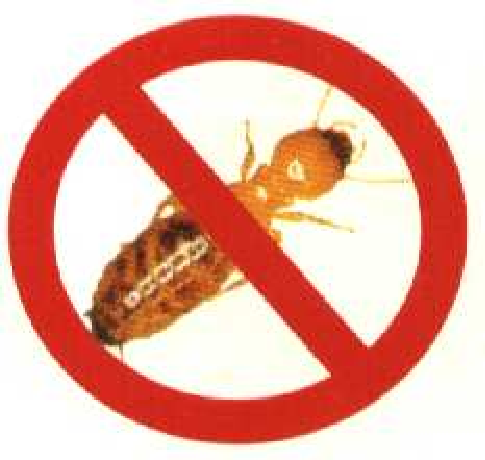
\includegraphics[width=0.5\textwidth]{Cap1/cupim}
\caption{Proibido estacionar cupins. Legenda grande, com o objetivo de demonstrar a indentação na lista de figuras.}
\label{cupim}
\end{figure}

Controle do manipulador após uma falha é fundamental do ponto de vista de operação, principalmente nos casos descritos acima, em que a localização do manipulador impede sua manutenção de forma fácil. Recentemente tem havido a combinação
de algorítmos de detecção e isolação de falhas com os de controle pós-falha em um método unificado. Uma extensão desse trabalho, que vê o problema de controle tolerante a falhas através de uma perspectiva integrada, foi proposta por
{marcel4}. Os autores apresentam um ambiente híbrido consistindo de três unidades básicas que garantem a compleição de tarefas na presença de qualquer número de juntas falhas (Figura \ref{cupim}). A primeira unidade é um esquema de detecção
e isolação de falhas que continuamente monitora o manipulador para detectar e identificar possíveis falhas nas juntas. A segunda unidade é responsável pela reconfiguração do controle. A terceira unidade é composta de algorítmos de
controle apropriados para cada tipo de configuração do robô, baseado na informação da unidade de reconfiguração \cite{COFFEE2000}.

No presente trabalho nos concentramos na unidade de algorítmo de controle, e mais especificamente no problema de controle da posição  angular de uma junta falha para qualquer posição desejada de uma maneira subótima, quando dispomos
de redundância de atuação para a realização dessa tarefa. O termo subótimo se deve ao fato de que não há garantias de otimalidade em vista das não-linearidades inerentes ao sistema e de outros fatores que serão abordados nos capítulos posteriores. Ao longo do texto, para simplificação, usaremos tanto o termo subótimo como ótimo para nos referirmos à metodologia utilizada.

Segundo, o critério de otimização utilizado será o acoplamento entre as juntas do
manipulador e neste caso, temos um sistema redundante quando ocorre falha de uma das juntas do manipulador de três juntas, e seu posicionamento é controlado pelas duas restantes. Nossa solução para o problema é baseada na formulação
de redundância local, extensivamente estudada no contexto de cinemática inversa ({nakamura}). A principal contribuição deste trabalho é a extensão deste método usando as equações dinâmicas de manipuladores subatuados e a utilização do índice de acoplamento como um critério para a minimização do torque e da energia gasta pelo sistema durante o controle das juntas falhas.

\begin{figure}[ht!]
\centering
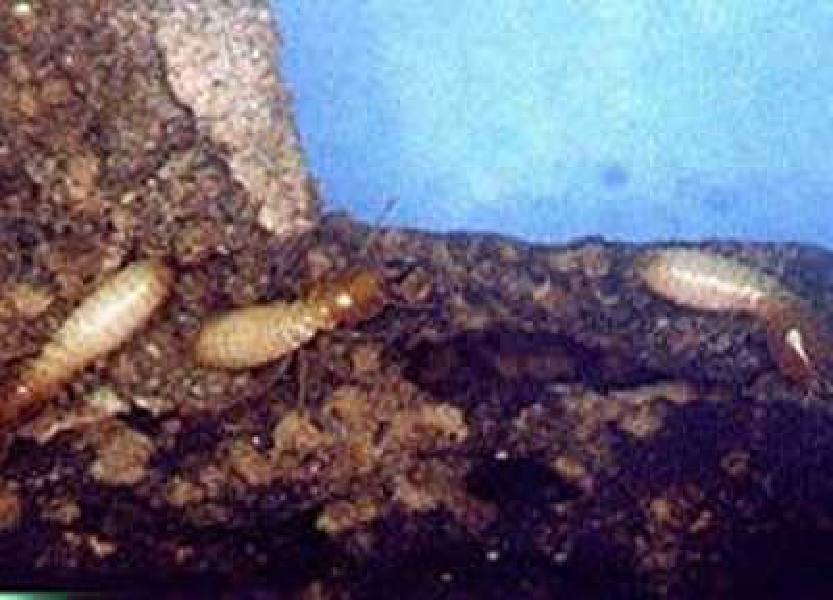
\includegraphics[width=1\textwidth]{Cap1/cupimconcreto}
\caption{Exemplo real de cupim frente ao seu dilema.}
\label{FDII}
\end{figure}

\section{Organização do trabalho}
\subsection{Sub-organização}
O capítulo 1 contém a introdução do trabalho, onde são expostos o objetivo, a motivação do mesmo, a descrição do sistema e a formulação do problema com a nomenclatura utilizada; além de uma revisão bibliográfica da literatura relacionada ao tema do trabalho.

\subsubsection{SubSub-organização}

No capítulo 2 apresentamos a modelagem dinâmica de um manipulador subatuado e o conceito de índice de acoplamento para medir o acoplamento dinâmico entre as juntas ativas e passivas. Este índice é utilizado para a análise e projeto de uma metodologia de controle subótimo do manipulador.

\subsubsection{Outra subsub-organizacao}

O capítulo 3 apresenta o controle subótimo de manipuladores através de redundância de atuação. Descreve-se a técnica de controle ponto a ponto de manipuladores subatuados. A seguir mostramos  a linearização destes por realimentação, cujo efeito é linearizar e desacoplar o sistema não linear. Finalmente é proposta uma sequência de controle subótimo local das juntas passivas visando a minimização de certos critérios como torque, velocidade e em particular a energia consumida pelo sistema. Este é de fato o tema principal deste mestrado.

É também apresentado no capítulo 4 um resumo do projeto de controladores  $H_{2}$ e $H_{\infty}$, cuja principal vantagem é a robustez na presença de incertezas paramétricas e distúrbios externos.

O capítulo 5 mostra as características e a operação do robô e do ambiente de simulação utilizados nos testes e experimentação da metodologia apresentada.

Os procedimentos da metodologia e os resultados obtidos para algumas configurações e diferentes controladores encontram-se no capítulo 6.

No capítulo 7 são apresentadas as conclusões do trabalho.

Quatro apêndices fazem parte do trabalho. O apêndice A apresenta alguns tópicos de álgebra linear que são a base do método proposto. No apêndice B são mostradas as equações da matriz de inércia e do vetor de torques não-inerciais
utilizados na modelagem dinâmica do manipulador. No apêndice C temos as expressões literais dessas equações feitas no software MAPLE e no apêndice D alguns programas feitos no software MATLAB utilizados no projeto \cite{Furmento1995}\cite{Morgado2003}.




% REFERENCIAS BIBLIOGRAFICAS
\renewcommand\bibname{\itareferencesnamebabel} %renomear título do capítulo referências
\bibliography{referencias}

\annex
\chapter{Exemplo em WSDL}\label{anex:wsdl-example}
\begin{minted}{xml}
<?xml version="1.0" encoding="UTF-8"?>
<description xmlns="http://www.w3.org/ns/wsdl"
             xmlns:tns="http://www.tmsws.com/wsdl20sample"
             xmlns:whttp="http://schemas.xmlsoap.org/wsdl/http/"
             xmlns:wsoap="http://schemas.xmlsoap.org/wsdl/soap/"
             targetNamespace="http://www.tmsws.com/wsdl20sample">

<documentation>
  This is a sample WSDL 2.0 document.
</documentation>

<!-- Abstract type -->
  <types>
    <xs:schema xmlns:xs="http://www.w3.org/2001/XMLSchema"
               xmlns="http://www.tmsws.com/wsdl20sample"
               targetNamespace="http://www.example.com/wsdl20sample">
     <xs:element name="Error" type="Error"/>
     <xs:element name="Pet" type="Pet"/>
     <xs:element name="Pets" type="Pets"/>
     <xs:element name="NewPet" type="NewPet"/>

     <xs:element name="ListPetsRequest" type="ListPetsRequest"/>
     <xs:element name="ShowPetByIdRequest" type="ShowPetByIdRequest"/>

     <xs:complexType name="Error">
      <xs:attribute name="code" type="xs:int"/>
      <xs:attribute name="message" type="xs:string"/>
     </xs:complexType>
     <xs:complexType name="Pet">
      <xs:attribute name="id" type="xs:int"/>
      <xs:attribute name="name" type="xs:string"/>
      <xs:attribute name="tag" type="xs:string" nillable="true"/>
     </xs:complexType>
     <xs:complexType name="NewPet">
      <xs:attribute name="name" type="xs:string"/>
      <xs:attribute name="tag" type="xs:string" nillable="true"/>
     </xs:complexType>
     <xs:complexType name="Pets">
      <xs:sequence>
        <xs:element minOccurs="0" name="pets" type="tns:Pet"/>
      </xs:sequence>
     </xs:complexType>

     <xs:complexType name="ListPetsRequest">
      <xs:attribute name="limit" type="xs:int" nillable="true"/>
      <xs:attribute name="cursor" type="xs:string" nillable="true"/>
     </xs:complexType>

     <xs:complexType name="ShowPetByIdRequest">
      <xs:attribute name="id" type="xs:int"/>
     </xs:complexType>
    </xs:schema>
  </types>

<!-- Abstract interfaces -->
  <interface name="PetStoreInterface">
    <fault name="Error1" element="tns:Error"/>
    <operation name="ListPets" pattern="http://www.w3.org/ns/wsdl/in-out">
      <input messageLabel="In" element="tns:ListPetsRequest"/>
      <output messageLabel="Out" element="tns:Pets"/>
    </operation>
    <operation name="CreatePet" pattern="http://www.w3.org/ns/wsdl/in-out">
      <input messageLabel="In" element="tns:NewPet"/>
      <output messageLabel="Out" element="tns:Pet"/>
    </operation>
    <operation name="ShowPetById" pattern="http://www.w3.org/ns/wsdl/in-out">
      <input messageLabel="In" element="tns:ShowPetByIdRequest"/>
      <output messageLabel="Out" element="tns:Pet"/>
    </operation>
  </interface>

<!-- Concrete Binding Over HTTP -->
  <binding name="HttpBinding" interface="tns:PetStoreInterface"
           type="http://www.w3.org/ns/wsdl/http">
    <operation ref="tns:ListPets" whttp:method="GET"/>
    <operation ref="tns:CreatePet" whttp:method="POST"/>
    <operation ref="tns:ShowPetById" whttp:method="GET"/>
  </binding>

<!-- Concrete Binding with SOAP-->
  <binding name="SoapBinding" interface="tns:PetStoreInterface"
           type="http://www.w3.org/ns/wsdl/soap"
           wsoap:protocol="http://www.w3.org/2003/05/soap/bindings/HTTP/"
           wsoap:mepDefault="http://www.w3.org/2003/05/soap/mep/request-response">
    <operation ref="tns:Get" />
    <operation ref="tns:CreatePet" />
    <operation ref="tns:ShowPetById" />
  </binding>

<!-- Web Service offering endpoints for both bindings-->
  <service name="PetStoreService" interface="tns:PetStoreInterface">
    <endpoint name="HttpEndpoint"
              binding="tns:HttpBinding"
              address="http://www.example.com/rest/"/>
    <endpoint name="SoapEndpoint"
              binding="tns:SoapBinding"
              address="http://www.example.com/soap/"/>
  </service>
</description>
\end{minted}


\chapter{Exemplo em OpenAPI}\label{anex:openapi-example}
\begin{minted}{yaml}
openapi: "3.0.0"
info:
  version: 1.0.0
  title: Swagger Petstore
  license:
    name: MIT
servers:
  - url: http://petstore.swagger.io/v1
paths:
  /pets:
    get:
      summary: List all pets
      operationId: listPets
      tags:
        - pets
      parameters:
        - name: limit
          in: query
          description: How many items to return at one time (max 100)
          required: false
          schema:
            type: integer
            format: int32
      responses:
        200:
          description: An paged array of pets
          headers:
            x-next:
              description: A link to the next page of responses
              schema:
                type: string
          content:
            application/json:
              schema:
                $ref: "#/components/schemas/Pets"
        default:
          description: unexpected error
          content:
            application/json:
              schema:
                $ref: "#/components/schemas/Error"
    post:
      summary: Create a pet
      operationId: createPets
      tags:
        - pets
      responses:
        201:
          description: Null response
        default:
          description: unexpected error
          content:
            application/json:
              schema:
                $ref: "#/components/schemas/Error"
  /pets/{petId}:
    get:
      summary: Info for a specific pet
      operationId: showPetById
      tags:
        - pets
      parameters:
        - name: petId
          in: path
          required: true
          description: The id of the pet to retrieve
          schema:
            type: string
      responses:
        200:
          description: Expected response to a valid request
          content:
            application/json:
              schema:
                $ref: "#/components/schemas/Pets"
        default:
          description: unexpected error
          content:
            application/json:
              schema:
                $ref: "#/components/schemas/Error"
components:
  schemas:
    Pet:
      required:
        - id
        - name
      properties:
        id:
          type: integer
          format: int64
        name:
          type: string
        tag:
          type: string
    Pets:
      type: array
      items:
        $ref: "#/components/schemas/Pet"
    Error:
      required:
        - code
        - message
      properties:
        code:
          type: integer
          format: int32
        message:
          type: string
\end{minted}


\chapter{Exemplo em Protocol Buffers}\label{anex:protobuf-example}
\begin{minted}{protobuf}
syntax = "proto3";

import "google/protobuf/empty.proto";

package petstore;

// Interface exported by the server.
service PetStoreService {
  // List all pets.
  rpc ListPets(ListPetsRequest) retuns (ListPetsResponse);

  // Create a pet.
  rpc CreatePet(CreatePetRequest) returns (google.protobuf.Empty);

  // Info for a specific pet.
  rpc ShowPetById(ShowPetByIdRequest) returns (Pet);
}

message ListPetsRequest {
  // How many items to return at one time (max 100).
  optional uint32 limit = 1;
  // A link to the page of responses
  optional string cursor = 2;
}

message ListPetsResponse {
  // A paged array of pets
  repeated Pet pets = 1;
  // A link to the next page of responses
  optional string cursor = 2;
}

message CreatePetRequest {
  string name = 2;
  optional string tag = 3;
}

message ShowPetByIdRequest {
  // The id of the pet to retrieve
  uint64 id = 1;
}

message Pet {
  uint64 id = 1;
  string name = 2;
  optional string tag = 3;
}
\end{minted}



% Glossario
%\itaglossary
%\printglossary

% Folha de Registro do Documento
% Valores dos campos do formulario
\FRDitadata{25 de março de 2015}
\FRDitadocnro{DCTA/ITA/DM-018/2015} %(o número de registro você solicita a biblioteca)
\FRDitaorgaointerno{Instituto Tecnológico de Aeronáutica -- ITA}
%Exemplo no caso de pós-graduação: Instituto Tecnol{\'o}gico de Aeron{\'a}utica -- ITA
\FRDitapalavrasautor{Cupim; Cimento; Estruturas}
\FRDitapalavrasresult{Cupim; Dilema; Construção}
%Exemplo no caso de graduação (TG):
\FRDitapalavraapresentacao{Trabalho de Graduação, ITA, São José dos Campos, 2015. \NumPenultimaPagina\ páginas.}
%Exemplo no caso de pós-graduação (msc, dsc):
%\FRDitapalavraapresentacao{ITA, São José dos Campos. Curso de Mestrado. Programa de Pós-Graduação em Engenharia Aeronáutica e Mecânica. Área de Sistemas Aeroespaciais e Mecatrônica. Orientador: Prof.~Dr. Adalberto Santos Dupont. Coorientadora: Prof$^\textnormal{a}$.~Dr$^\textnormal{a}$. Doralice Serra. Defesa em 05/03/2015. Publicada em 25/03/2015.}
\FRDitaresumo{Sistemas Web apresentam um grau de complexidade bastante diversificado, variando desde
um sistema comercial de um mercado de bairro até o sistema completo de uma multi-nacional
em escala global. Para simplificar o desenvolvimento desses sistemas, diversas ferramentas
foram desenvolvidas.

Este trabalho apresenta um novo modelo de gerador de APIs, com o objetivo de solucionar
problemas que ferramentas atuais apresentam. Esses problemas são relacionados a baixa
integração com outras ferramentas de desenvolvimento, como Object-Relational Mappings
(ORMs) e validadores. Mostramos também que o uso de um gerador que integre eficientemente
com o restante do ecossistema pode resultar em grandes ganhos de eficiência para o time de
desenvolvimento, além de abrir portas para o uso de outras ferramentas que não seriam possíveis
sem ele. Uma motivação para esse trabalho é a busca do aumento de eficiência e automação dentro
do processo de desenvolvimento e a redução na incidência de defeitos em sistemas complexos.
}
%  Primeiro Parametro: Nacional ou Internacional -- N/I
%  Segundo parametro: Ostensivo, Reservado, Confidencial ou Secreto -- O/R/C/S
\FRDitaOpcoes{N}{O}
% Cria o formulario
%\itaFRD

\end{document}

% Fim do Documento. O massacre acabou!!! :-)
